\documentclass[a4paper,12pt]{report}

%
% Bunch of useful packages
%
\usepackage[utf8]{inputenc}
\usepackage{algorithmic}
\usepackage{algorithm}
\usepackage{pst-plot}
\usepackage{graphicx}
\usepackage{graphics}
\usepackage{floatflt}
\usepackage{wrapfig}
\usepackage{endnotes}
\usepackage{amsfonts}
\usepackage{amsmath}
\usepackage{amsthm}
\usepackage{amssymb}
\usepackage{verbatim}
\usepackage{hyperref}
\usepackage{multirow}
\usepackage{endnotes}
\usepackage{pdflscape}
\usepackage{multicol}
\usepackage{tikz}
\usetikzlibrary{arrows}
\usepackage{wrapfig}
\usepackage{hyperref}
\usepackage{array}
\usepackage{rotating}
\usepackage{enumitem}
\usepackage{setspace}
\usepackage{enumitem}

\usepackage[font={small, sl}]{caption}

%
% Listings
%
\usepackage{color}
\usepackage{xcolor}
\usepackage{listings}
\lstset{
	basicstyle=\scriptsize\ttfamily,
	numbers=left,
	numberstyle=\tiny,
	numbersep=5pt,
	tabsize=2,
	extendedchars=true,
	breaklines=true,
	keywordstyle=\color{red},
	frame=b,         
	stringstyle=\color{white}\ttfamily,
	showspaces=false,
	showtabs=false,
	xleftmargin=17pt,
	framexleftmargin=17pt,
	framexrightmargin=5pt,
	framexbottommargin=4pt,
	showstringspaces=false
}
\usepackage{caption}
\DeclareCaptionFont{white}{\color{white}}
\DeclareCaptionFormat{listing}{\colorbox{gray}{\parbox{\textwidth}{#1#2#3}}}
\captionsetup[lstlisting]{format=listing,labelfont=white,textfont=white}

%
% Chapter titles
%
\usepackage{titlesec}
\titleformat{\chapter}[hang] 
{\normalfont\huge\bfseries}{\thechapter}{1em}{} 

%
% Theorems and Definitions
%
\theoremstyle{definition}
\newtheorem{definition}{Definition}[chapter]

%
% Margins of all kinds
%
\hypersetup{pdfborder={0 0 0 0}}
\setlength\parindent{0mm}
\setlength\parskip{3mm}

\newenvironment{pitemize}{
\vspace{-5mm}
\begin{itemize}
 	\setlength{\itemsep}{1pt}
	\setlength{\parskip}{0pt}
 	\setlength{\parsep}{0pt}
}{
	\end{itemize}
	\vspace{-8mm}
}


%%%%%%%%%%%%%%%%%%%%%%%%%%%%%%
%% Width of A4 is 8.27in (210mm) We have an inside margin of 1.5 in and outside margin of 1in
%% This leaves 5.77in for text width
\oddsidemargin=0.5in
\evensidemargin=0.0in
\textwidth=5.77in
\headheight=0.0in
\topmargin=0.0in
\textheight=9.0in
%%%%%%%%%%%%%%%%%%%%%%%%%%%%%%


\newenvironment{sitemize}
{\vspace{-2mm}\begin{list}{\textbullet}{%
    \setlength{\itemsep}{0pt}%
    \setlength{\parsep}{0pt}%
    \setlength{\topsep}{0pt}%
    \setlength{\parskip}{0pt} %
    \setlength{\labelwidth}{0pt}%
    \setlength{\labelsep}{0.05in} %
    \setlength{\leftmargin}{5pt} %
    \renewcommand{\labelitemi}{\textbullet}}}
  {\vspace{-2mm}\end{list}}

\newenvironment{mitemize}
{\begin{list}{\textbullet}{%
    \setlength{\itemsep}{0pt}%
    \setlength{\parsep}{0pt}%
    \setlength{\topsep}{2mm}%
    \setlength{\parskip}{0pt} %
    \setlength{\labelwidth}{0pt}%
    \setlength{\labelsep}{0.05in} %
    \setlength{\leftmargin}{8.5mm} %
    \renewcommand{\labelitemi}{\textbullet}}}
  {\end{list}}


\newcommand\epigraph[3]{
\vspace{1em}\hfill{}\begin{minipage}{#1}{\begin{spacing}{0.9}
\small\noindent\textit{#2}\end{spacing}
\vspace{1em}
\hfill{}{#3}}\vspace{2em}
\end{minipage}}


%
% Title
%
% TODO title would better be a bit shorter

\begin{document}
\begin{center}
	{\Large
	University of Tartu\\
	Faculty of Mathematics and Computer Science\\
	Institute of Computer Science\\
	Computer Science\\}
	
	\vspace{2.5cm}
	
	{\LARGE Taivo Pungas}\\
	\vspace{0.5cm}
	\begin{spacing}{2}{\Huge\bf \ \ \ Unsupervised learning algorithms implemented by a biologically realistic neuron model}\end{spacing}
	\vspace{0.5cm}
	{\LARGE Bachelor's thesis (9 ECTS)}
\end{center}
\vspace{3cm}
\hspace{7.2cm}{\Large Supervisors: Dr. Raul Vicente\\}
\vspace{-0.5cm}

\hspace{10.4cm}{\Large Dr. Jaan Aru \\}

\ \\
\ \\
Author: .................................................. "......." May 2015\\
Supervisor: ............................................. "......." May 2015\\
\ \\
Approved for defense\\
Professor: ............................................... "......." May 2015\\
\ \\
\begin{center}
	{\Large Tartu 2015}
\end{center}
\thispagestyle{empty}
\pagebreak


%%%
% Abstract
%%%


{\textbf
{\Large Title of thesis in English}}

\textbf{Abstract:}

Lorem ipsum dolor sit amet, consectetur adipiscing elit. Etiam a ultricies sem, vel gravida dolor. Vestibulum lacinia nulla nec massa mollis eleifend. Etiam scelerisque erat in ligula dapibus, et eleifend enim vulputate. Integer quis lobortis neque, eget efficitur felis. Vestibulum vel consequat quam. Praesent volutpat eget massa rutrum fringilla. Maecenas fringilla turpis ut dignissim luctus. Nunc lectus metus, dapibus eu enim ut, rhoncus blandit ligula. Praesent gravida ullamcorper est id pharetra. Mauris tempus ornare sollicitudin. Sed feugiat nec turpis mattis sollicitudin. Aliquam non orci sit amet lorem rutrum euismod et non orci. Aliquam egestas aliquam blandit. Cras quis convallis neque. Integer fringilla pharetra condimentum. Fusce erat eros, pulvinar sit amet orci in, consectetur accumsan eros.

\textbf{Keywords:} taivo, raul, jaan, model, neuro, stuff

\vspace{1.5cm}



{\textbf
{\Large Töö eestikeelne pealkiri}}

\textbf{Lühikokkuvõte:}

Lorem ipsum dolor sit amet, consectetur adipiscing elit. Etiam a ultricies sem, vel gravida dolor. Vestibulum lacinia nulla nec massa mollis eleifend. Etiam scelerisque erat in ligula dapibus, et eleifend enim vulputate. Integer quis lobortis neque, eget efficitur felis. Vestibulum vel consequat quam. Praesent volutpat eget massa rutrum fringilla. Maecenas fringilla turpis ut dignissim luctus. Nunc lectus metus, dapibus eu enim ut, rhoncus blandit ligula. Praesent gravida ullamcorper est id pharetra. Mauris tempus ornare sollicitudin. Sed feugiat nec turpis mattis sollicitudin. Aliquam non orci sit amet lorem rutrum euismod et non orci. Aliquam egestas aliquam blandit. Cras quis convallis neque. Integer fringilla pharetra condimentum. Fusce erat eros, pulvinar sit amet orci in, consectetur accumsan eros.

\textbf{Võtmesõnad:} taivo, raul, jaan, mudel, neuro, värk


\
\thispagestyle{empty}
\pagebreak

\tableofcontents
\newpage


% % % %
% Chapter: Introduction
% % % %

\chapter*{Introduction}
\addcontentsline{toc}{chapter}{Introduction}

Your brain is a complex organ capable of very sophisticated thought. Even though the chess-playing supercomputer Deep Blue won the reigning world champion Garry Kasparov, Kasparov was also able to do anything human beings do every day, whereas the computer could only play chess. The human brain is remarkable not for its ability to do one particular thing very well, be it playing chess, reading an article in Nature, preparing a six-course meal, or slam dunking in a basketball game. It is remarkable for being able to do all of those things, and much more.

However, gaining understanding of the brain's information processing mechanisms remains one of the major scientific challenges today. A key aspect of the brain is \emph{neural plasticity}, its ability to change itself over time as new knowledge and experience are accumulated and processed. To understand the dynamics of these changes, computational models are explored to understand how well they explain the brain's behaviour as observed in experiments in neuroscience. To this end, it is useful to create models that are biophysically realistic, i.e. are guided by known biophysical principles of the brain's and neurons' structure.

Researching the brain has been a high priority in several large-scale projects. The Human Brain Project, funded by the European Union, is an attempt "to understand the human brain and its diseases, and ultimately to emulate its computational capabilities"\footnote{https://www.humanbrainproject.eu/vision}. The BRAIN Initiative, funded by the National Institutes of Health in the United States, focuses on "understanding how individual cells and complex neural circuits interact in both time and space"\footnote{http://braininitiative.nih.gov/index.htm}. TODO@Elena[is this kind of footnote OK?]. TODO this paragraph needs introductory and summarising sentences. From @Jaan[is this paragraph out of place?]

Major successes in creating systems with significant capacity for learning have recently been achieved using deep convolutional neural networks in tasks ranging from playing video games \cite{mnih2015human} to describing scenes in natural language \cite{karpathy2014deep}. The neuron models used in these systems are very simple, often composing of a scalar product of the inputs and weights, and a rectifying function. However, evidence from brains has shown that each neuron is a much more complex and powerful information processing unit.
From @Jaan[not happy with the current logical flow of the paragraphs]

This thesis explores the behaviour of one particular previously published (with a Nobel-winning physicist among the authors) biophysically realistic model in important information processing tasks. The model has been shown to produce a range of neural plasticity phenomena. This work explores the computational capabilities that arise from this unifying model of plasticity. In particular, the thesis investigates...


% % % %
% Chapter: Preliminaries
% % % %

\chapter{Background and related work}


\section{Overview of relevant neuroscience}
TODO 'relevant' is not the best word

% Biology of the human brain
\subsection{Neurobiology of the brain}
The brain, a part of the nervous system, is the central information processing organ in animals. The computational properties of the brain arise from the heavily interconnected networks and sub-networks of specialised cells called \emph{neurons}. It has been approximated \cite{herculano2009human} that the human brain consists of $10^{11}$ neurons with $10^{15}$ inter-neuronal connections called \emph{synapses}. This work focuses on modelling one of many different types of neurons - pyramidal neurons.


\subsection{Neurons as computational units}
Every model of a brain that aspires for biophysical reality must include a way to model the behaviour of neurons and synapses. Each neuron can be seen as a small unit performing computation on some inputs and producing corresponding output. There are many computational models of neurons, with the level of detail ranging from complex multi-compartment models to very simple models such as those used in many artificial neural networks (ANNs). 

\begin{figure}[h]
    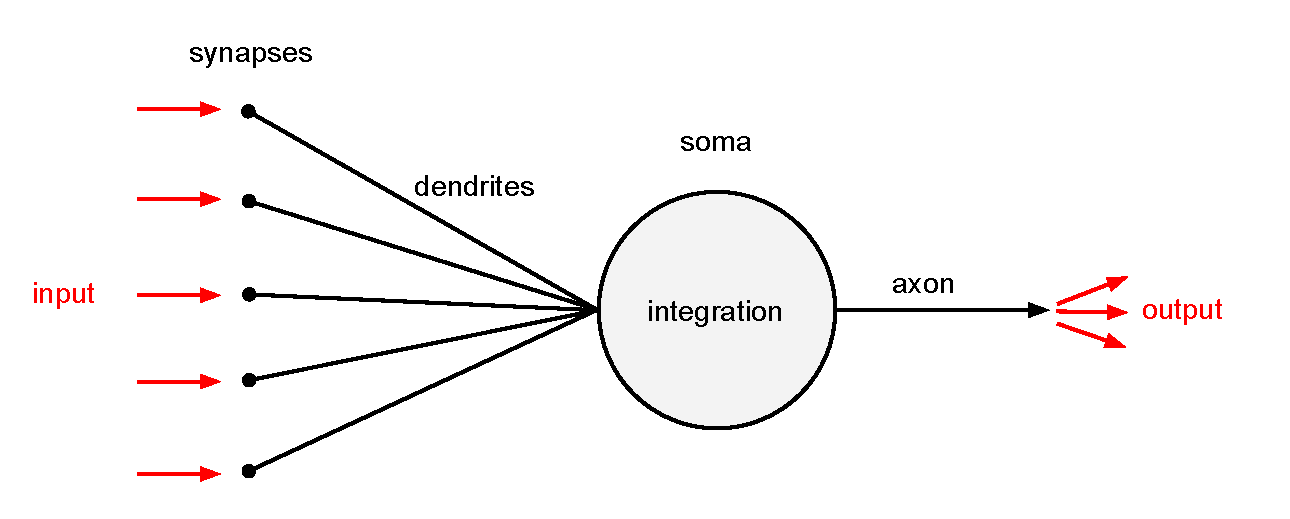
\includegraphics[width=\textwidth]{fig1}
    \caption{Schematic of a pyramidal neuron.}
    \label{fig:pyramidal}
\end{figure}

Information flow through a neuron follows a path from the inputs to the output, with integration of information in between, as shown in Figure~\ref{fig:pyramidal}.


\subsubsection{Input}
%Where does the input come from? How is it encoded (spikes)?
%The number of inputs to a pyramidal neuron can range from $x$ to $x$ (cite) depending on (what?). 

The region of connection between two neurons is called a \emph{synapse}, with information flowing from the axon of the \emph{presynaptic} neuron to a dendrite of the \emph{postsynaptic} neuron. Each time the presynaptic neuron produces significant output, neurotransmitters are released from the presynaptic neuron into the \emph{synaptic cleft}, a small gap between the presynaptic and postsynaptic neurons at the synapse.
Neurotransmitters then bind to receptors on the dendrite of the postsynaptic neuron, causing ion channels to open. This causes ion flow across the membrane, which causes a voltage change at the dendrite of the postsynaptic neuron.

Synapses can be divided into two classes: input arriving at \emph{excitatory} synapses tends to increase the output of the postsynaptic neuron, input to \emph{inhibitory} synapses tends to make it fire less.

%How does information about a spike reach the postsynaptic neuron, aka how do synapses work? Neurotransmitters and detectors. What happens when post-neuron detects neurotransmitters (explain in terms of ions and voltage)? 

\subsubsection{Computation}
A single neuron can be viewed as an integrator of information over time, over different inputs, or both. At each synapse, a neuron has some intrinsic biological components that determine how much this synapse should affect the output of the postsynaptic neuron. \emph{Synaptic weights} are key parameters used in modelling such biological components, and the modification of synaptic weights is the basis of learning in neurons.

After the contribution of input from each synapse is computed, this information must be integrated to produce the output of the neuron. Different models of information integration exist. Different neural models of information integration exist. Some of the best known, from least to most detailed, are the McCulloch-Pitts (MP), Integrate-and-Fire (IF), and Hodgkin-Huxley (HH) models. In the MP model which is widely utilised in ANNs, a weighted sum of inputs is calculated, to which a sigmoid function is applied to produce the output of the neuron. In the IF and HH models the neuron is modelled as an electric circuit, and then corresponding differential equations are used to calculate the output of the neuron.

\subsubsection{Output}

Output of a neuron takes the form of \emph{action potentials} or (TODO 'or' is not good here) \emph{spikes}, rapid increases in membrane voltage followed by a return to the equilibrium voltage.

Information about action potentials is conducted from a neuron to the dendrites of other neurons using the axon. Axons are usually not part of single neuron models as the output of the modelled neuron is studied in and of itself, so needs not be relayed to other neurons.

\section{Prior work}
TODO Suggestions from Elena: more detail (obv), examples of published models, what I do differently, why I chose this particular model. Add references.


There are many computational models of neurons, with the level of detail ranging from compartmental to very simple models of a neuron such as those used in ANNs. Using these models, it is possible to simulate neurons in a computer and investigate the models' behaviour in a very controlled and detailed way. As opposed to real experiments that are hindered by many difficulties, using a simulation approach allows detailed investigation and control of input and all parameters.


\subsection{Models of neural information integration}

%\subsection{Single neuron models}
%The model I am using was originally published in \cite{shouval2002unified}. The model is good because all parts of the model have biological interpretations, so the model can be said to be biophysically realistic.

The perceptron \cite{rosenblatt1958perceptron} that works as a simple linear classifier was one of the earliest proposed computational models of the neuron. Since then, numerous models have been proposed. An important characteristic of a neuron model is its mechanism of learning, However, few models explicitly model the biochemistry and physiology leading to synaptic plasticity.




\subsection{Models of neural plasticity}

Different kinds of possible learning rules. Simple ones such as Hebb's rule, Oja's rule, BCM theory. What properties these rules have been shown to have (what behaviours they produce -- PCA etc). Finding learning rules by minimising Fisher information, other information-theoretic measures, or some other objective function \cite{echeveste2014generating}.
The neuron modelled in this work utilises a slightly modified version (TODO modified in what way?) of a calcium-based model of bidirectional synaptic plasticity proposed in \cite{shouval2002unified} and \cite{yeung2004synaptic}.


\subsection{Single neuron models in unsupervised learning tasks}
Oja rule, BCM rule, etc have been shown to do PCA/ICA etc. Tempotron has been shown. Yeung 2004 showed selectivity. But seems that most work about unsupervised learning focuses on networks, not biophysical single neurons.

The tempotron \cite{gutig2006tempotron} models neuron, but includes components whose biophysical accuracy is not well grounded (finding locations with maximum voltage). UNSUP learning was done on this.


% % % %
% Chapter: Methods
% % % %
\chapter{Methods}
\section{Neuron model used}

The neuron model used in this work follows the Ca\textsuperscript{2+}-based model of a single neuron published in \cite{shouval2002unified} and \cite{yeung2004synaptic}. An integrate-and-fire model of information integration is used, and no dendritic distance is simulated, i.e. the possibility that some synapses are further from the soma than others is not taken into account. Details are shown in ref [shouval 2002 and the one before]. Here, an overview of the most important aspects of the model will be given.

\subsubsection{Input generation}
Inputs to the model are simulated as $N$ spike trains, one for each synapse, with a given mean firing rate $r$ specified independently for each synapse. The spike trains are produced in a homogeneous Poissonian process, i.e. the occurrence of a spike is independent of the time since the last spike, and the average rate of spikes remains constant. Uncorrelated inputs are generated using TODO CITE (HomoPoisSpikeGen function)?
Correlation between inputs is simulated by specifying the correlation parameter $0 \leq c \leq 1$, and using code from \cite{macke2009} to generate correlated homogeneous Poissonian spike trains.

\subsubsection{Synapse}
describe how input spike trains are translated into EPSPs/IPSPs

The release of neurotransmitters caused by each presynaptic spike is assumed to last 1 ms.

\subsubsection{Integrate-and-fire model}

The voltage of the postsynaptic neuron can be increased by excitatory postsynaptic potentials (EPSPs) caused by presynaptic spikes at excitatory synapses, and decreased due to inhibitory postsynaptic potentials (IPSPs) caused by presynaptic spikes at inhibitory synapses. In addition, a leak current is simulated, which tends to return voltage to the resting potential.

When postsynaptic voltage $V_{post}$ reaches the threshold $V_{thres}$, a postsynaptic spike is generated by rapidly increasing $V_{post}$ to the spiking voltage $V_{spike}$. Then, $V_{post}$ is returned to the reset potential $V_{reset}$, from where it returns to the baseline voltage.

Each EPSP is a sum of two decaying exponentials, normalised to have a desired amplitude. The EPSP-s of all synapses are summed linearly and no dendritic distance is simulated in this model. Upon a postsynaptic spike, $BPAP(t)$ is set to its peak voltage $V_{amplitude_{BPAP}}$, and then starts to decay as a sum of a slow component (time constant $\tau_f$) and a fast component (time constant $\tau_s$).

$$ EPSP(t) = ? $$
$$ BPAP(t) = ? $$

FIGURE: spatial and temporal summation of EPSP-s, causing a spike (action potential) vs not causing a spike.



\subsubsection{Learning}


TODO use Shouval Scholarpedia article for explaining basis of learning (http://www.scholarpedia.org/article/Models_of_synaptic_plasticity#Calcium_dependent_models_of_bidirectional_synaptic_plasticity)

Coincidence detector

%There are two possible sources of increase in the dendritic voltage of the postsynaptic neuron: excitatory postsynaptic potentials (EPSPs) caused by presynaptic spikes at excitatory synapses and back-propagating action potentials (BPAPs) caused by the postsynaptic neuron firing. Postsynaptic voltage can decrease due to inhibitory postsynaptic potentials (IPSPs) caused by presynaptic spikes at inhibitory synapses, or passive decay that tends to return voltage to the resting potential.

It is assumed that different forms of depolarisation (EPSP and BPAP) add linearly. 

Inhibitory synapses are not plastic.

Differential equation for updating weights: $$ \frac{dW_j}{dt} = \eta ([Ca]_j) (\Omega([Ca]_j) - W_j)$$

FIGURES of important functions (eta, omega)




\section{Implementation details}

Timestep, other important parameters? Mention here maybe complexity of the program, the bugs I've found, the time window in which input is generated, what values parameters are initialised to (voltage, m,n,h etc).

The model is implemented in MATLAB. Source code is freely available under the [CC BY-SA?] license at [link].


% % % %
% Chapter: Results
% % % %
\chapter{Results}
\section{Validation of the implementation}

% Figures 3A, 3B, 3C from Shouval 2002. Maybe should move to Results > Validation?
FIGURE: mean final weight vs clamped postsynaptic voltage (for 100 presynaptic pulses at low frequency)

FIGURE: mean final weight vs input rate

FIGURE: STDP curve (normalised mean final weight vs post-pre timing)


\section{Unsupervised learning task}
Show that our model does PCA/ICA

Simulation results showing that the model implements algorithms

\subsection{Simulation protocol}




\section{Probability of release?}

\section{Inhibitory plasticity?}


% % % %
% Chapter: Discussion
% % % %
\chapter{Discussion}



% % % %
% Appendices
% % % %
\chapter*{Appendix A: Description of model parameters}
\addcontentsline{toc}{chapter}{Appendix A: Description of model parameters}

possibly add a table of parameters with their values and descriptions here

\chapter*{Appendix B: MATLAB code}
\addcontentsline{toc}{chapter}{Appendix B: MATLAB code}

link to github, also say that will be attached as supplementary material (see Julius's thesis)


% % % %
% Glossary
% % % %
\chapter*{Glossary}
\addcontentsline{toc}{chapter}{Glossary}
ANN - artificial neural network
EPSP
IPSP
BPAP
STDP
PCA
ICA


% % % %
% Bibliography
% % % %

\bibliographystyle{alpha}
\addcontentsline{toc}{chapter}{Bibliography}
\bibliography{Thesis}
Internet URLs were valid on May 14, 2015.
\newpage


% % % %
% License
% % % %

\chapter*{License}
\addcontentsline{toc}{chapter}{License}


%
% Non-exclusive license to reproduce thesis and make thesis public
%
\section*{Non-exclusive license to reproduce thesis and make thesis public}
I, Ilya Kuzovkin (09.07.1988), 
\begin{enumerate}
	\item herewith grant the University of Tartu a free permit (non-exclusive licence) to:
	\begin{enumerate}[label*=\arabic*.]
		\renewcommand{\theenumi}{\arabic{enumi}}
		\item reproduce, for the purpose of preservation and making available to the public, including for addition to the DSpace digital archives until expiry of the term of validity of the copyright, and
		\item make available to the public via the web environment of the University of Tartu, including via the DSpace digital archives until expiry of the term of validity of the copyright,
	\end{enumerate}
	``A New Approach to Training Brain-Computer Interface Systems", supervised by Konstantin Tretyakov,
	
	\item I am aware of the fact that the author retains these rights.

	\item I certify that granting the non-exclusive licence does not infringe the intellectual property rights or rights arising from the Personal Data Protection Act. 
\end{enumerate}

Tartu, 20.05.2013

\thispagestyle{empty}
\newpage

\end{document}






















